\subsection{A fixed classifier: examples versus positive predictions}
\label{sec:classification}
Consider a fixed two-label classifier with whole-example abstention. Exposure $W$ counts its positive predictions, and loss $L$ counts false positives, so $1-R$ is accepted micro-precision. Three contexts have the following known conditional moments:
\[
\begin{array}{c|ccc}
 &K&U&V\\\hline
 \Pr(X)&2/5&2/5&1/5\\
 h(X)&(1,0)&(1,0)&(1,1)\\
 w(X)&1&1&2\\
 \ell(X)&0&3/10&1/2
\end{array}
\]
At risk cap $r=1/10$ and case floor $c_0=7/20$, every optimum accepts $K$. Its risk surplus funds the remaining constraint $4a_U+3a_V\leq2$. Maximizing accepted examples chooses $(a_K,a_U,a_V)=(1,1/2,0)$, giving $(c,d_W)=(3/5,1/2)$. Maximizing accepted positive predictions instead chooses $(1,0,2/3)$, giving $(8/15,5/9)$. Both attain exactly 90\% micro-precision. The classifier is unchanged; only the value assigned to acceptance differs (Figure~\ref{fig:mechanism}). Appendix~\ref{app:classification} specifies the label distribution and verifies both optima.

For ordinary binary precision, accepting all predicted-negative cases costs no risk budget, and completed gates satisfy $c=1-T+Td_W$. Both objectives then have a common optimum. This contrast makes the acceptance unit consequential: gating each label separately would change the multi-label problem above.

\begin{figure}[t]
\centering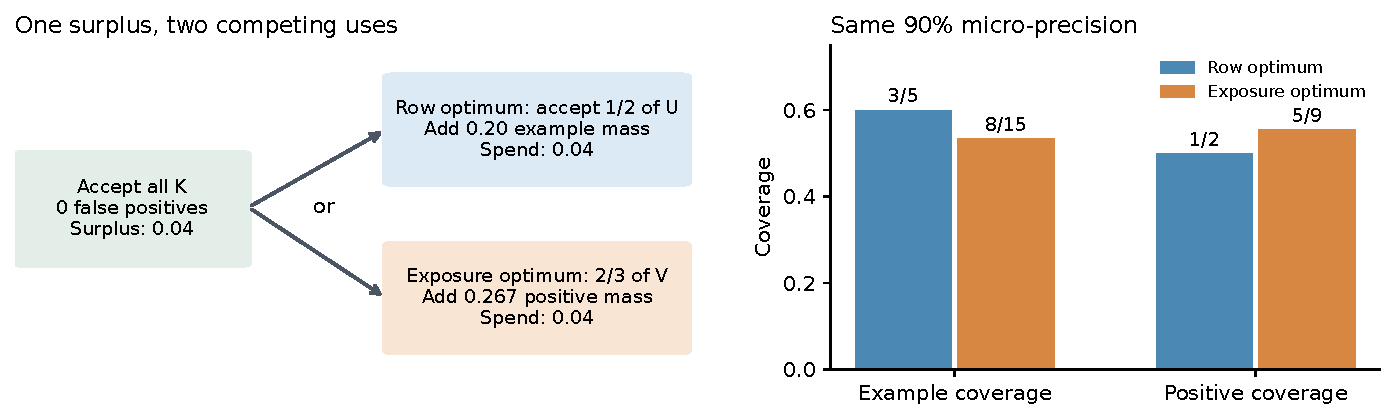
\includegraphics[width=\linewidth]{figures/utility_mechanism.pdf}
\caption{Exact fixed-classifier example, not an empirical benchmark. Left: the accurate context $K$ supplies 0.04 expected excess units; either competing allocation uses all of them. Right: the same risk budget buys more examples or more positive predictions, but not both. Fractional acceptance is independent randomization within a context.}
\label{fig:mechanism}
\end{figure}
